\documentclass[final,hyperref={pdfpagelabels=false}]{beamer}
\usepackage[size=custom,orientation=landscape,width=88,7,height=116,2,scale=1.0]{beamerposter}
\usetheme{I6pd2}
\usepackage[utf8]{inputenc}
\usepackage[frenchb]{babel}
\usepackage{amsmath,amsthm,amssymb,latexsym}
\usepackage{times}\usefonttheme{professionalfonts}
\usefonttheme[onlymath]{serif}
\usepackage{booktabs}
\graphicspath{{figures/}}
\usecaptiontemplate{\small\structure{ }\insertcaption}
\usepackage{multicol}
\usepackage{subfigure}
\setbeamercolor{background canvas}{bg=taaluminium,fg=taaluminium}
%%%%%%% TITLE SECTION %%%%%%%
\title{\huge  Object Removal by Exemplar-Based Inpainting \small Based on Criminisi work}
\author{Di Folco Maxime, GIrot Charly, Jallais Maëllis}
\institute{Ecole Supérieure de Chimie Physique Électronique de Lyon}
%%%%%%%% FOOTER %%%%%%%%
\newcommand{\leftfoot}{\textbf{References} : \hfill \break 
* Criminisi et al : Region filling and object removal by exemplar based image inpainting. IEEE Transactions on image processing, 2004 \hfill \break
*Bertalmio et al, Image Inpainting. Proceedings of the 27th annual conference on Computer graphics and interactive techniques, 2000.  }
\newcommand{\rightfoot}{maxime.di-folco@cpe.fr \\ charly.girot@cpe.fr \\ maeliss.jallais@cpe.fr}


\begin{document}
\addtobeamertemplate{block end}{}{\vspace{2ex}}
\begin{frame}[t]

%%%%%%%% INTRODUCTION %%%%%%%%
\begin{columns}[t]
\begin{column}{.02\textwidth} \end{column}
\begin{column}{.930\textwidth} 
\begin{block}{Introduction *,**}
\begin{columns}[t]
\begin{column}{.496\textwidth}
Objectif
\begin{itemize} 
\item \textbf{Supprimer des objets large} définis par l'utilisateur, à partir d'images numériques. 
\item Corrections d'artefacts ou Restauration d'image
\item Rendu réaliste ou vraisemblable pour l'œil humain
\end{itemize}
Principe
\begin{itemize} 
\item Remplir des régions masquées, par \textbf{propagation de texture} le long des structures linéaires 
\item Utilisation du Principe de \textbf{connectivité} pour définir l'ordre de remplissage : propager les textures tout en conservant les structures linéaires de l'image
\item Recherche de \textbf{patch similaire} par analyse couleur
\end{itemize}

Historique / État de l'art 

 


\end{column}
\begin{column}{.496\textwidth}
\begin{figure}[!b]
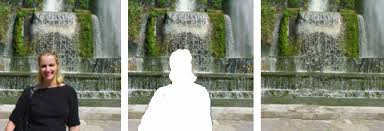
\includegraphics[width=0.8\linewidth]{inpaintingex.jpeg}
\caption{Exemple. De gauche à droite. Originale, Suppression de la région, Remplissage de textures. }
\label{example}
\end{figure}
\end{column}
\end{columns}
\end{block}
\end{column}


\begin{column}{.02\textwidth} \end{column}
\end{columns}

\begin{columns}[t]

\begin{column}{.02\textwidth} \end{column}

\begin{column}{.465\textwidth} 


\begin{block}{Méthode}
Respect du principe de connectivité et les 3 points de l'algo 
Algorithme en 3 étapes 
\begin{itemize}
\item Calcul des priorités en bordure du masque
\begin{itemize}
\item Terme de données * Confiance
\item Terme de données : Quantité de variation des textures autour du pixel courant
\item Confiance : importance accordée au pixel courant
\end{itemize}
figures exemples avec les ovales 
\item Propager texture et information structurelle
\begin{itemize}
\item La priorité est donnée aux zones de fortes variations (terme de données)
\item Propager la texture en commencant par ses zones permet de conserver les structures linéaires de l'image
\item les données de textures manquantes autour du pixel de plus forte priorité sont issues de la zone de l'image la plus ressemblante (SSD dans l'espace couleur Lab)
\end{itemize}
figures exemples avec le test priority carre si on a un truc pas trop moche en résultat 
\item Mise à jour de la confiance : les nouveaux pixels copiés obtiennent la confiance du pixel courant de sorte que sa valeur diminue vers l'intérieur du masque indiquant l'incertitude sur la valeur du pixel
\end{itemize}

figures d'actualisation de la confiance 
\end{block}

\begin{block}{Résultats}


résultat sur les ovales , sur le test priority, sur des vrais images 


\end{block}
\end{column}


\begin{column}{.465\textwidth}
\begin{block}{Discussion}
Ce qui a marché et comment dans quelles limites 
l'imporatnce de la taille du patch 
Les limitiations de notre algo : la montgolfiere , les patchs opposés ? 
les bordures dans notre implémentation,
Amélioration possible
une interface graphique pour séléctionner les zones qui vont bien a la main par l'utilisateur 
zone de recherche du patch ... 
\end{block}
\end{column}


\end{columns}
\end{frame}
\bibliographystyle{\small}
\end{document}